\documentclass[a4paper]{report}

\usepackage[greek, english]{babel}
\usepackage[utf8]{inputenc}
\usepackage{amsmath}
\usepackage{graphicx}
\usepackage[colorinlistoftodos]{todonotes}
\usepackage{tikz}
\usetikzlibrary{shapes,arrows}
\usepackage{verbatim}

\newcommand{\inlinecode}{\texttt}

\title{DP1 Proposal -- psax}

\author{Will Oursler}

\date{\today}

\begin{document}
\maketitle

\section{Overview}

The proposed system extends UNIX systems to implement ``search folders'': curated directories created from queries for contents and file attributes. While users typically create directories based on shared attributes of files in them, current file-systems do not allow for definition of directories based on these attributes. Extending the UNIX file-system to support this model of use will make it more powerful and intuitive.

I propose responsive but efficient daemon (loosely modeled after the popular UNIX tool \inlinecode{cron}). It is assumed that search folders lagging a few minutes behind the system in day to day usage is acceptable but if a user mounts a new search folder then it must immediately be available for use once the process used to initialize it terminates.

In the spirit of \inlinecode{cron}'s name being derived from \textgreek{χρόνος} for time, \inlinecode{psax} is derived from \textgreek{f'aximo}, greek for search or investigation. 

\section{Design Description}

\subsection{Usage Example}

A photographer wants to create a folder of all her recent pictures (e.g. pictures taken in the last 3 days). She runs the command

\begin{center}
\inlinecode{searchmount "\textasciitilde/Recent Pictures" \textasciitilde/Pictures -mtime -3}
\end{center}

The mounted folder will always contain symlinks of the pictures from the last 3-4 days (the extra day is because \inlinecode{psax} will only recheck files it has confirmed match the query about once a day). If at any later date she puts a new batch of pictures in any subdirectory of \inlinecode{ \textasciitilde/Pictures } then symlinks will appear within a few minutes.

\begin{figure}[h!]
  \centering
  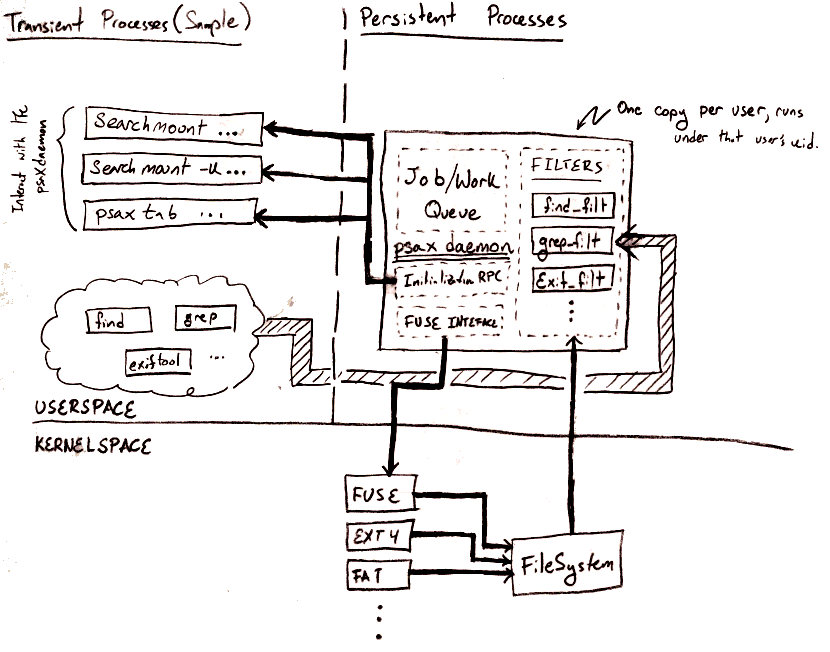
\includegraphics[width=1.0\textwidth]{image}
  \caption{A rough overview of the modules involved in \inlinecode{psax} and their interconnections. Notice that the processes that the user interacts with (\inlinecode{searchmount}, \inlinecode{psaxtab}) are wrappers on a \inlinecode{psaxdaemon} API.}
\end{figure}

\subsection{Requirements and Overhead}

\inlinecode{psax} is designed to run in userspace with minimal kernel modification\footnote{\inlinecode{psax} uses \inlinecode{FUSE} -- Filesystem in Userspace -- to avoid modifying kernel code. FUSE is prepackaged in many package repositories, so it not an onerous requirement.}. Each user is responsible for maintaining their own table of descriptions of search folders (a \inlinecode{psaxtab}). A userspace daemon (the \inlinecode{psaxdaemon}) is responsible for ensuring that these descriptions are properly mounted and maintained.

It is assumed that when a \inlinecode{searchmount} command is run, it is acceptable that the \inlinecode{psaxdaemon} briefly consume a moderate amount of CPU, but during everyday use, the daemon cannot use many system resources, even at the (potential) expense of latency.

\subsection{Storage}

Because our searches are expensive, \inlinecode{psaxdaemon} saves the results in a persistent database on disk. In parallel with the FUSE interface, we will store this as a linked list. One table will hold a mapping from directory names to the full path of first relevant file. Subsequently, each filename can be used to retrieve the next relevant result. These databases are maintained by the daemon and persist over reboots, so examining the contents of a search folder has minimal overhead.

\subsection{Use of \inlinecode{inotify}}

To ensure that relevant new files are quickly discovered, \inlinecode{inotify} is used. When a new \inlinecode{searchmount} command is issued, directories of interest (and their subdirectories) are added to inotify.

However, there are many special cases we must consider. Because \inlinecode{inotify} does not issue alerts for subdirectories, special care will need to be taken to ensure that the directory structure is properly maintained.

\subsection{Timing}

Efficiency is a central concern. The \inlinecode{psaxdaemon} is susceptible to load spikes; moving or copying directories may create more work for \inlinecode{psax} than can be done immediately.

For this reason, the \inlinecode{psaxdaemon} will maintain a queue of jobs, along with estimations of the CPU time required to complete them. The daemon is responsible for choosing when to run these tasks to ensure that the CPU load is kept low.

\subsection{Filters}

While we initially want to support the same sorts of queries as GNU \inlinecode{find}, it is likely that we might want to issue other sorts of queries. We may wish to issue queries related to
\begin{itemize}
\item The content of ASCII encoded files. \inlinecode{find} does not include functionality for this, other utilities like \inlinecode{grep} do.
\item The times and locations in which photos were taken. These are often encoded in EXIF data included in files.
\end{itemize}

Filters support a wide array of different queries. A filter is a small piece of code available to the \inlinecode{psaxdaemon}. It provides an API so that each filter may be run on a single file, a directory of files (but not its subdirectories - the \inlinecode{psaxdaemon} will schedule them separately), and quick estimates of how long each of these tasks will take may be obtained. Each filter takes a user-specified context as an argument. In the case of \inlinecode{find\_filter}, this context would be the set of flags the user would use with \inlinecode{find}.

\section{Conclusion}

I have proposed an implementation of search folders with minimal overhead and almost no modifications existing systems. This system will provide users with a more intuitive and versatile file system. Problems remain to be solved in the course of implementation - primary those related to the interface with FUSE: how, for instance, we will deal with multiple relevant files with the same name remains heretofore unsolved. I am confident that these are minor issues that can be sensibly resolved in the proposed framework with further consideration.

\section{References}

J. Saltzer  and  M. Kaashoek,  \textit{Principles  of  Computer  System  Design:  An  Introduction}.
Burlington,  MA:  Morgan  Kaufmann,  2

FUSE Project, \textit{fuse.sourceforge.net/}

inotify manual page, \textit{man7.org/linux/man-pages/man7/inotify.7.html}



\end{document}